%\documentclass[handout]{beamer}
\documentclass{beamer}
\usepackage{algorithm2e}
\usepackage{natbib}
\usepackage{layouts}
%\usepackage{enumitem}
%\usepackage[dvipsnames]{xcolor}
\definecolor{vuborange}{rgb}{1.0,0.40,0.0}
\definecolor{forestgreen}{rgb}{0.13, 0.55, 0.13}
\usetheme{Boadilla}
\usepackage{color,soul}
\usepackage{xcolor}
\usepackage{adjustbox}
\usepackage{amsmath,amssymb}
\usepackage{tikzsymbols}
\usepackage{booktabs}
\usepackage{calc}
\usepackage{subcaption}
\usepackage{graphicx}
\usepackage{tikz}
\usepackage{tikz-qtree}

%\newcommand\citet[1]{\citeauthor{#1}~\citeyear{#1}}
\usepackage[bordercolor=white,backgroundcolor=gray!30,linecolor=black,colorinlistoftodos]{todonotes}
\newcommand{\rework}[1]{%
	\todo[color=yellow,inline]{Rework: {#1}}%
}

\usetikzlibrary{shapes.geometric, arrows}

\title{Toward human-interpretable explanations using Machine Learning for explanation generation}
\institute[shortinst]
{\inst{1} DataLab, Vrije Universiteit Brussel, Belgium \\ % Your institution for the title page
	\inst{2} DTAI, KULeuven, Belgium \\ % Your institution for the title page
	\inst{1}\{firstname.lastname\}@vub.be, \inst{2}\{firstname.lastname\}@kuleuven.be
}
\date{DTAI Seminar 2023}
\author{\underline{Emilio Gamba}\inst{1, 2} \and Ignace Bleukx \inst{2} \and  Jo Devriendt\inst{2} \and Dimos Tsouros\inst{2} \and  Bart Bogaerts\inst{1} \and   Tias Guns\inst{1,2}}

\newcommand\hlyellow[1]{\hl{ {\sethlcolor{yellow}#1}}}
\newcommand\hlgreen[1]{\sethlcolor{green}\hl{#1}}

\tikzstyle{startstop} = [rectangle, rounded corners, minimum width=2cm, minimum height=0.5cm,text centered, draw=black]
\tikzstyle{io} = [trapezium, trapezium left angle=70, trapezium right angle=110, minimum width=3cm, minimum height=1cm, text centered, draw=black, fill=blue!30]
\tikzstyle{process} = [rectangle, minimum width=3cm, minimum height=1cm, text centered, draw=black, fill=orange!30]
\tikzstyle{decision} = [diamond, minimum width=3cm, minimum height=1cm, text centered, draw=black, fill=green!30]
\tikzstyle{arrow} = [thick,->,>=stealth]


\newcommand\m[1]{\ensuremath{\mathcal{#1}}\xspace}
\newcommand\allconstraints{\m{T_P}}
\newcommand\theory{\ensuremath{\m{F} }\xspace}
\newcommand\formula{\ensuremath{\m{F} }\xspace}
\newcommand\formulac{\ensuremath{\m{C} }\xspace}
\renewcommand\emph[1]{{\color{vuborange}#1}}
\newcommand\Iend{\m{I_{\mathit{end}}}}
\newcommand\Ipartial{\m{I}}
\newcommand\factexpl{fact\xspace}
\newcommand\LitsToExplain{DigitToExplain}

\newcommand\nat{\m{\mathbb{N}}}
\newcommand\subsetT{\m{\mathcal{S}}}
\newcommand\ltrue{\m{\textbf{t}}}
\newcommand\lfalse{\m{\textbf{f}}}
\newcommand\call[1]{\m{\textsc{#1}}}
\newcommand\onestep{\call{OneStep}}

\newcommand\muses[1]{\textsc{mus}s(\m{#1})}
\newcommand\mcses[1]{\textsc{mcs}s(\m{#1})}
%\begin{frame}{How to find OCUSs?}
%
%	
%\end{frame}

\newcommand\setstohit{\m{\mathcal{H}}}
\newcommand\grow{\call{Grow}}
\newcommand\sat{\call{SAT}}
\newcommand\corrss{\call{Correction-Subsets}}
\newcommand\comus{\call{ocus}}
\newcommand\cohs{\call{CondOptHittingSet}}
% \renewcommand{\labelitemi}{$\triangleright$}
\renewcommand{\thealgocf}{}


\makeatletter
\renewcommand{\@algocf@capt@plain}{above}% formerly {bottom}
\setbeamertemplate{footline}
{
	\leavevmode%
	\hbox{%
		\begin{beamercolorbox}[wd=.2\paperwidth,ht=2.25ex,dp=1ex,center]{author in head/foot}%
			\usebeamerfont{author in head/foot}Emilio Gamba (VUB)
		\end{beamercolorbox}%
		\begin{beamercolorbox}[wd=.5\paperwidth,ht=2.25ex,dp=1ex,center]{title in head/foot}%
			\usebeamerfont{title in head/foot}Toward human-interpretable explanations
		\end{beamercolorbox}%
		\begin{beamercolorbox}[wd=.3\paperwidth,ht=2.25ex,dp=1ex,center]{date in head/foot}%
			\usebeamerfont{date in head/foot}DTAI Seminar 2023\hspace*{1em}
			\insertframenumber{} / \inserttotalframenumber\hspace*{2ex} 
	\end{beamercolorbox}}%
	\vskip0pt%
}
\makeatother

\begin{document}
	
	\begin{frame}
		\maketitle
		\begin{minipage}{0.45\textwidth}
			\begin{flushleft}
				
\includegraphics[width=\textwidth]{template_vub/VUB-AI_RGB-1-800x223}
			\end{flushleft}
		\end{minipage}		\hfill
	\begin{minipage}{0.15\textwidth}
	
	
\includegraphics[width=\textwidth]{figures/DTAI_Logo_2}
\end{minipage}
\hfill
	\begin{minipage}{0.15\textwidth}
		
		
\includegraphics[width=0.7\textwidth]{figures/datalab_400x400.jpg}
	\end{minipage}
	\end{frame}
	
	
%	\AtBeginSection[]
%	{
%		\begin{frame}
%			\frametitle{Outline}
%			\tableofcontents[currentsection]
%		\end{frame}
%	}
%	
%	\AtBeginSubsection[]
%	{
%		\begin{frame}
%			\frametitle{Outline}
%			\tableofcontents[currentsection,currentsubsection]
%		\end{frame}
%	}
%	

		\begin{frame}
\tableofcontents
	
\end{frame}			
	\begin{frame}
		
		\setlength{\textfloatsep}{0pt}
		\frametitle{Examples of Constraint Satisfaction Problems}
		\begin{minipage}[t]{0.45\textwidth}
			\begin{figure}[h]
				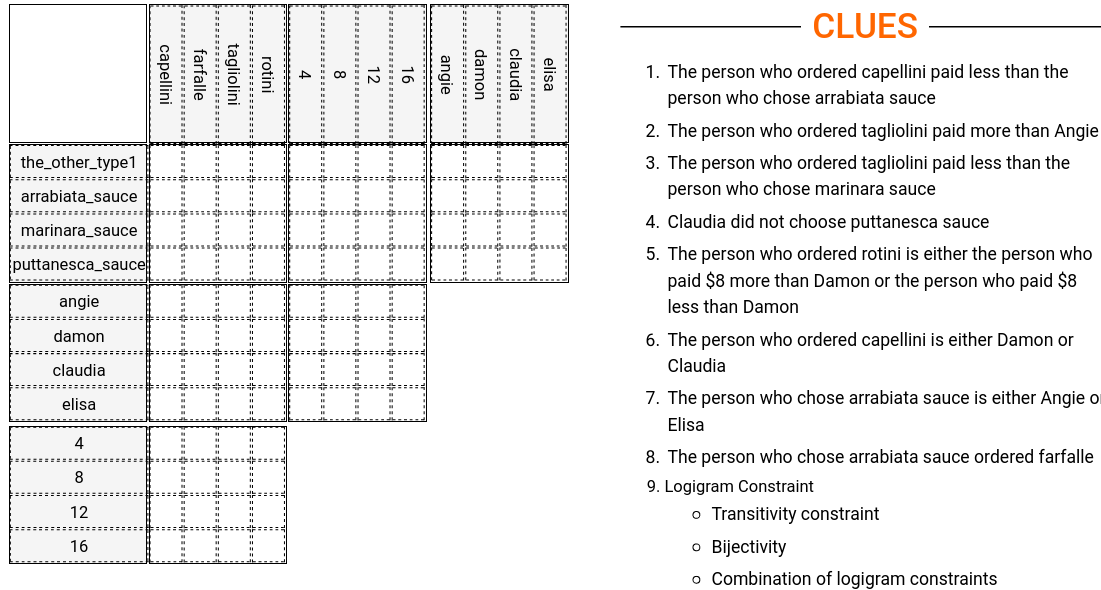
\includegraphics[width=\textwidth]{figures/logic_puzzle.png}
				\caption{\small Logic Grid Puzzle}
			\end{figure}
				\vspace{-8mm}
			\begin{figure}[h]
				\centering
				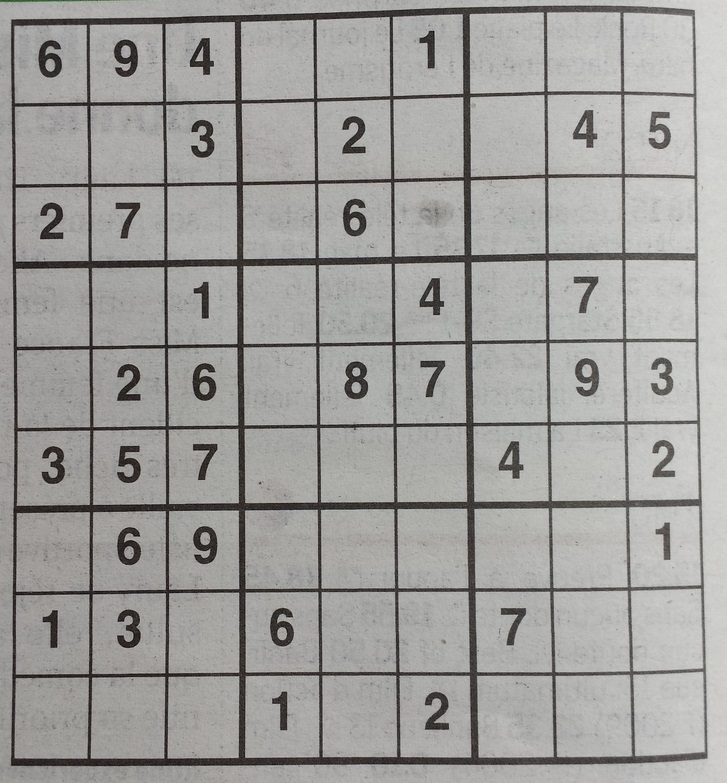
\includegraphics[width=.6\textwidth]{figures/sudoku_steps/sudoku.jpg}
				\caption{\small Sudoku}
			\end{figure}
		\end{minipage}
		\hfill
		\begin{minipage}[t]{0.52\textwidth}
			\begin{figure}[h]
				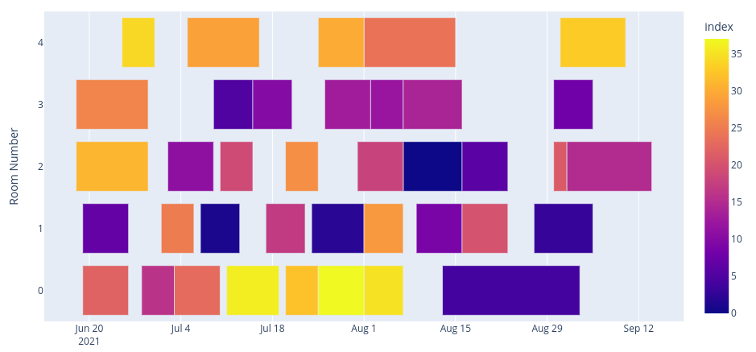
\includegraphics[width=\textwidth]{figures/scheduling.png}
				\caption{\small (Room) Scheduling Problem}
			\end{figure}
				\vspace{-8mm}
			\begin{figure}[h]
				\includegraphics[width=\textwidth]{figures/omus-presentation-car.png}
				\caption{\small (Car) configuration problems}
			\end{figure}
		\end{minipage}

	\end{frame}
	
	\section{Motivation}
\begin{frame}
	\frametitle{Constraint Satisfaction Problems}
	\framesubtitle{Solving}
	
	\begin{center}
		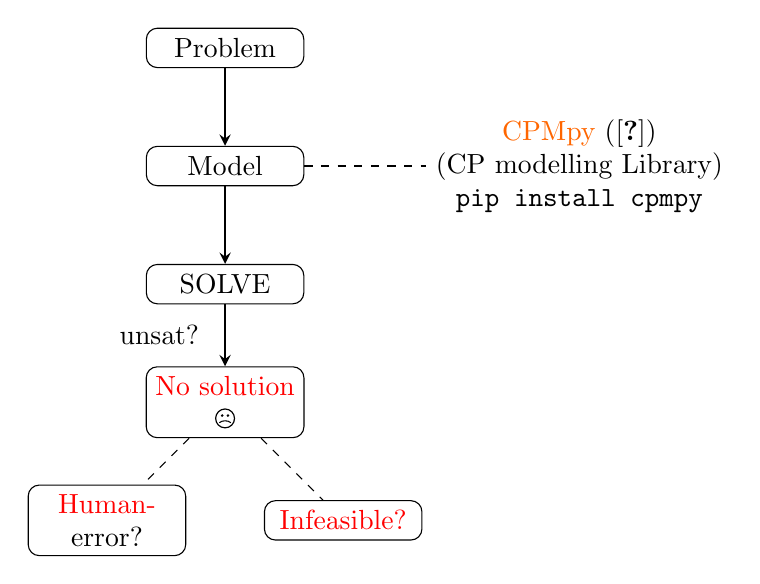
\begin{tikzpicture}[node distance=1.5cm]
			\node (problem) [startstop] {Problem};
			\pause
			\node (model) [startstop, below of=problem] {Model}; 
			\draw [arrow] (problem) -- (model);			
%			\node (Essence) [right of=model, xshift=1cm] {CPMpy \cite{CPMpy}}; 
			\node (cpmpy) [align=center, right of=model, xshift=3cm] {\emph{CPMpy} (\cite{guns2019increasing}) \\ (CP modelling Library) \\\texttt{pip install cpmpy}}; 
%			\node (Essence) [right of=model, xshift=1cm] {CPMpy \cite{CPMpy}}; 
			\draw [dashed] (model) -- (cpmpy);									
			\pause
			
			\node (solve) [startstop, below of=model] {SOLVE};
			\draw [arrow] (model) -- (solve); \pause
			
			\node  (modelerror) [startstop, below of=solve, align=center] {\color{red} No solution\\ \Sadey}; %todo: add smiley face sad
			\draw [arrow] (solve) --node[anchor=east,xshift=-0.2cm] {unsat?} (modelerror); 			
			\pause
			\node  (human) [startstop, below of=modelerror, xshift=-1.5cm, align=center] {\color{red} Human-\\error?}; %todo: doodle human
			\draw [dashed] (modelerror) --  (human); 
			\pause
			\node  (Infeasible) [startstop, below of=modelerror, xshift=1.5cm, align=center] {\color{red} Infeasible?}; 
			\draw [dashed] (modelerror) --  (Infeasible); 

		\end{tikzpicture}
	\end{center}
\end{frame}

\begin{frame}
	\frametitle{Constraint Satisfaction Problems}
	\framesubtitle{Solving}
			\begin{minipage}{0.4\textwidth}
		\begin{center}
			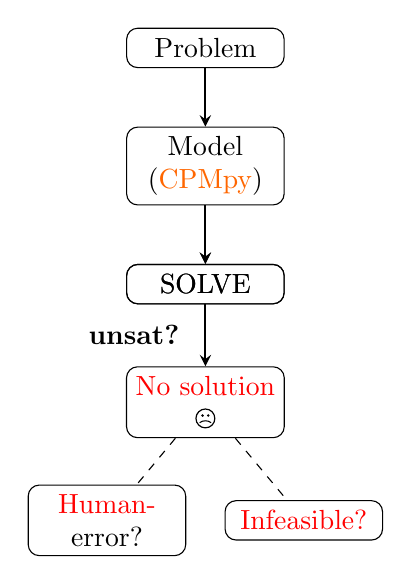
\begin{tikzpicture}[node distance=1.5cm]
				\node (problem) [startstop] {Problem}; 
				
				\node (model) [startstop, below of=problem,align=center] {Model \\ (\emph{CPMpy})}; 
				\draw [arrow] (problem) -- (model);			
				
%				\node (cpmpy) [right of=model, xshift=0.75cm] {CPMpy}; 
%				\draw [dashed] (model) -- (cpmpy);									
				
				\node (solve) [startstop, below of=model] {SOLVE};
				\draw [arrow] (model) -- (solve); 
			
			\node (solve) [startstop, below of=model] {SOLVE};
			\draw [arrow] (model) -- (solve); 

			\node  (modelerror) [startstop, below of=solve, align=center] {\color{red} No solution\\ \Sadey}; %todo: add smiley face sad
			\draw [arrow] (solve) --node[anchor=east,xshift=-0.2cm] {\textbf{unsat?}} (modelerror); 			
			\node  (human) [startstop, below of=modelerror, xshift=-1.25cm, align=center] {\color{red} Human-\\error?}; %todo: doodle human
			\draw [dashed] (modelerror) --  (human); 
			\node  (Infeasible) [startstop, below of=modelerror, xshift=1.25cm, align=center] {\color{red} Infeasible?}; 
			\draw [dashed] (modelerror) --  (Infeasible); 

				\end{tikzpicture}
		\end{center}
	\end{minipage}
	\begin{minipage}{0.59\textwidth}
	\textbf{How do you explain UNSAT ? } \\	
	\begin{figure}[H]
		\centering
	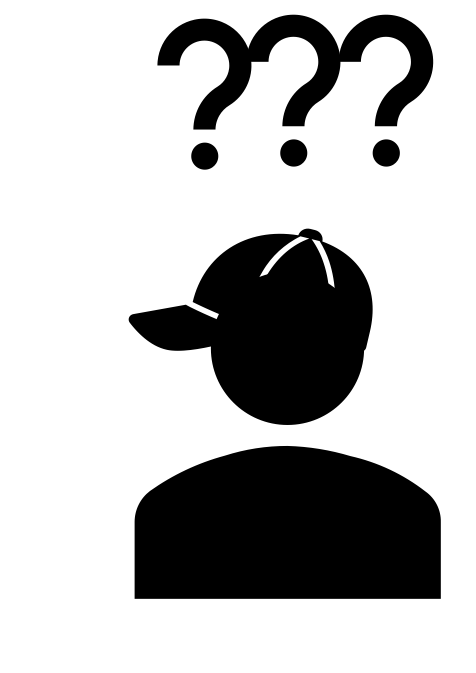
\includegraphics[width=0.3\textwidth]{figures/unsat/human.png}
	\end{figure}

%	\pause
%	\begin{itemize}
%		\item Extract a \emph{Minimum Unsatisfiable Subsets} (MUS) \pause
%		\item Enumerate all \emph{Minimum Unsatisfiable Subsets} (MUS) \pause
%		\item Extract a \emph{Minimum Correction Subsets} (MCS)
%		\begin{itemize}
%			\item \emph{Correct} your model by modifying a subset of the model constraints
%		\end{itemize}
%	\end{itemize}
	\end{minipage}
\end{frame}

\begin{frame}
	\frametitle{How do I debug my model}
	\framesubtitle{Explanations of unsatisfiability}
	

\begin{minipage}{0.7\textwidth}
	\only<1>{\hfill}
	 \only<2->{
\begin{enumerate}
	\item Identify conflicting constraints as an explanation  \footnotesize{(\cite{DBLP:journals/jar/LiffitonS08,ignatiev2015smallest}...)}
	\begin{itemize}
		\item[$\rightarrow$] Extract a \textbf{\textit{\color{red}Minimum Unsatisfiable Subset}} (\textbf{\textit{\color{red}MUS}}) 
		\item[=] Irreducible Inconsistent Subsystem (ISS) 
	\end{itemize}
 \only<3->{\item Identify a \textbf{\textit{\color{forestgreen}Maximal Satisfiable Subset}} (\textbf{\textit{\color{forestgreen}MSS}}) {\footnotesize{(\cite{ignatiev2019rc2,davies2013exploiting,hansen1990algorithms}...)}}} 
\only<4->{\item ``Correct'' the infeasibility in the constraints \footnotesize{(\cite{liffiton2013enumerating}...)}
	\begin{itemize}
	\item[$\rightarrow$] Extract a \textbf{\textit{\color{blue}Minimum Correction Subset}} (\textbf{\textit{\color{blue}MCS}})
	\item[=] Complement of some \textbf{\textit{\color{forestgreen}MSS}}, removal/correction leads to a satisfiable subset
\end{itemize}}
\end{enumerate}}

		\end{minipage}
	\begin{minipage}{0.28\textwidth}
	\only<1>{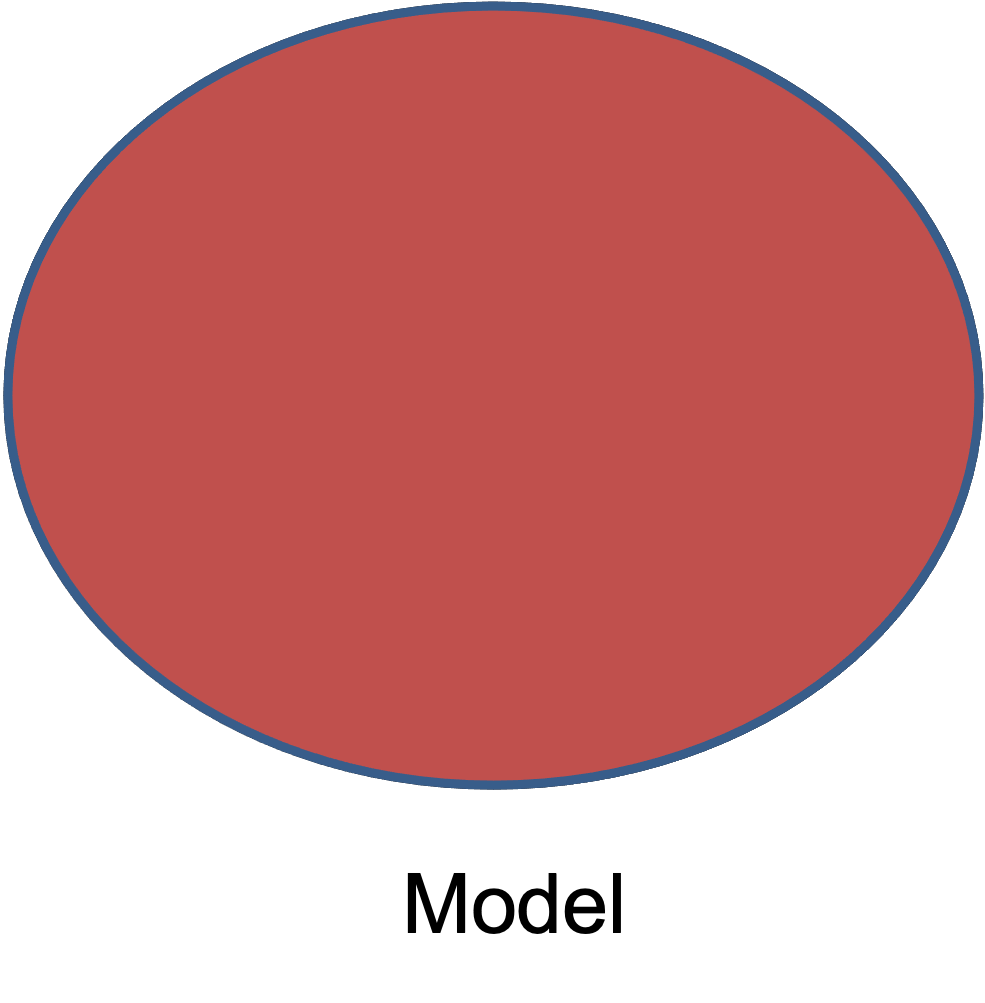
\includegraphics[width=\textwidth]{figures/unsat/model.png}}
	\only<2>{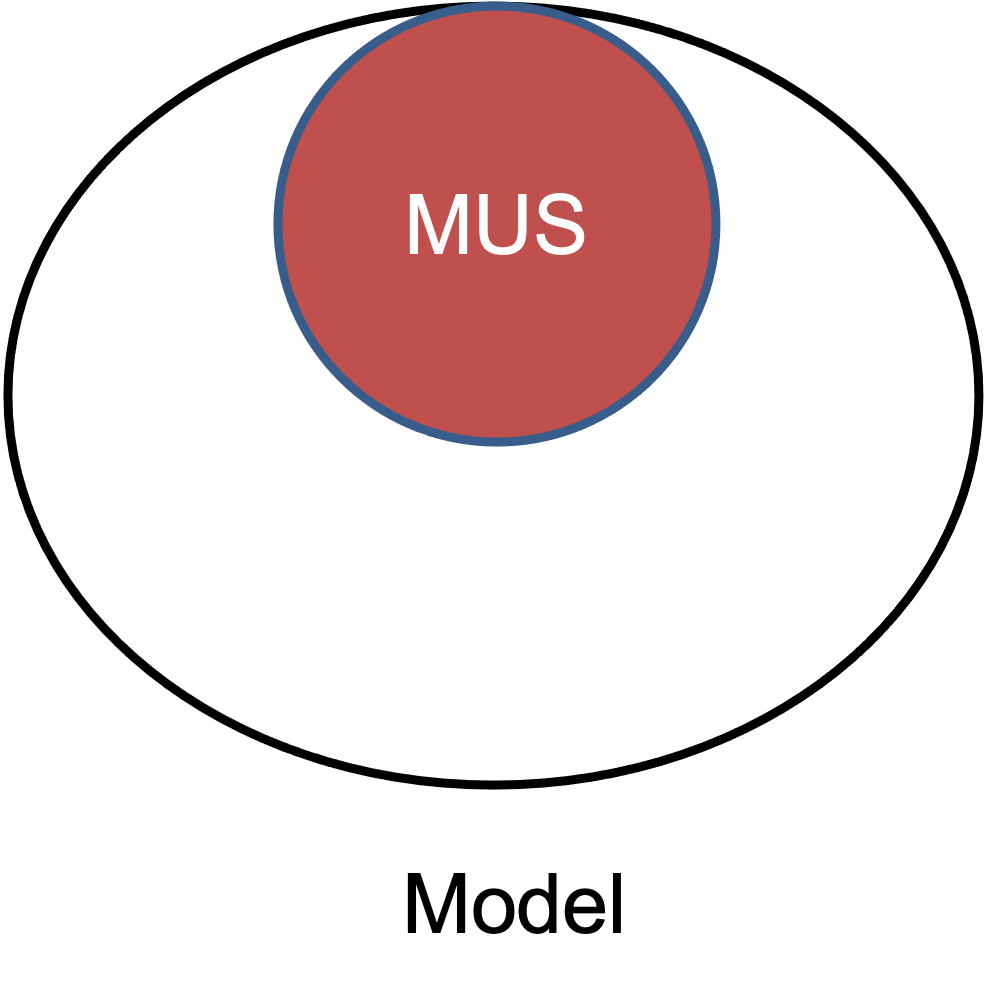
\includegraphics[width=\textwidth]{figures/unsat/mus.png}}
	\only<3>{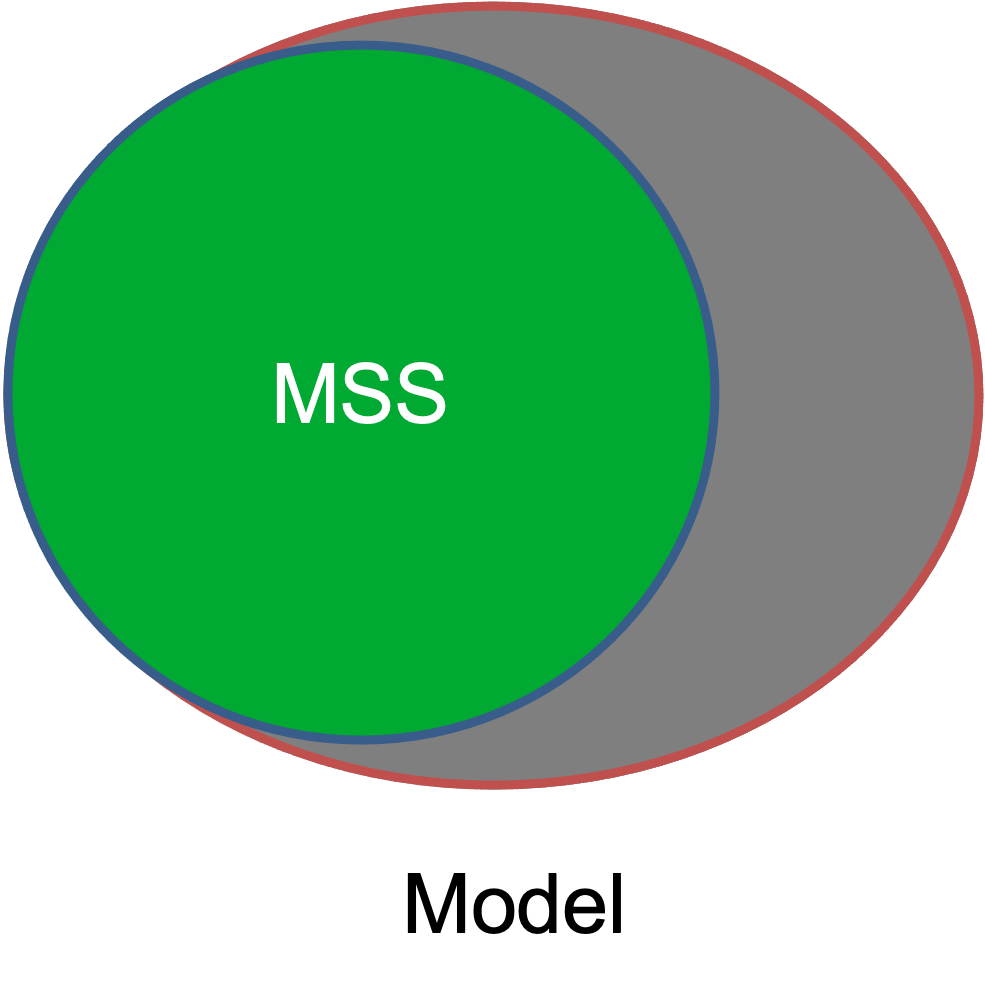
\includegraphics[width=\textwidth]{figures/unsat/mss.png}}
	\only<4>{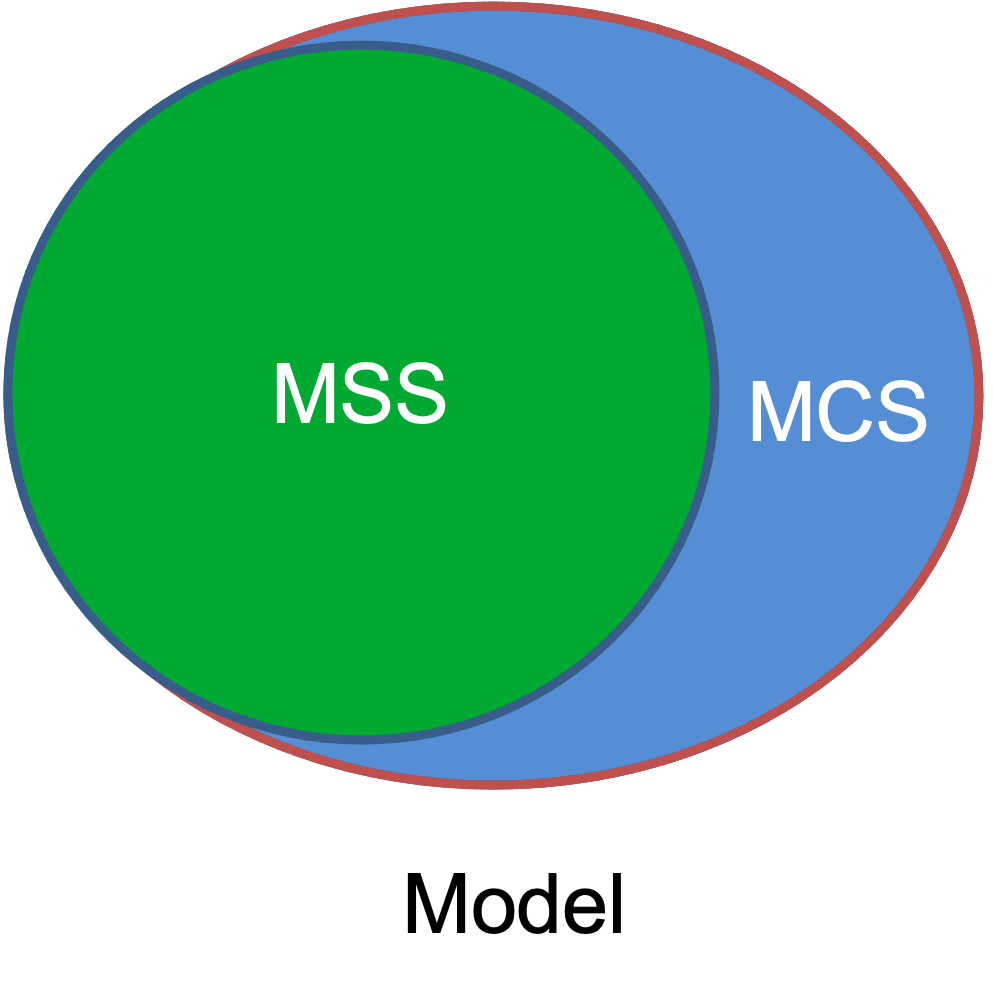
\includegraphics[width=\textwidth]{figures/unsat/msc.png}}
	\end{minipage}
\vfill
\end{frame}
	
	\section{How do I explain Satisfiability?}
	\begin{frame}
		\frametitle{Motivation - Explaining SAT problems}
		\begin{minipage}{0.35\textwidth}
			\begin{center}
				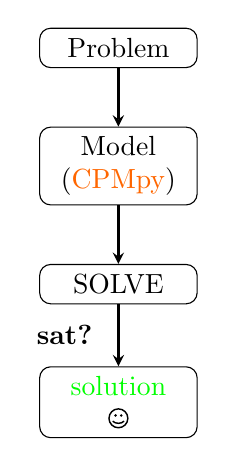
\begin{tikzpicture}[node distance=1.5cm]
					\node (problem) [startstop] {Problem}; 
					
				\node (model) [startstop, below of=problem,align=center] {Model \\ (\emph{CPMpy})}; 
				\draw [arrow] (problem) -- (model);								
					
					\node (solve) [startstop, below of=model] {SOLVE};
					\draw [arrow] (model) -- (solve); 
					
					%					\node  (modelerror) [startstop, below of=solve] {\color{red} modeling error?};
					%					\draw [arrow] (solve) --node[anchor=east,xshift=-0.2cm] {unsat?} (modelerror); 
					\node  (solution) [startstop, below of=solve,align=center]  {\color{green} solution\\ \Smiley};
					%						\node  (solution) [startstop, below of=sat] {\color{green} solution};
					%	
					\draw [arrow] (solve) --node[anchor=east,xshift=-0.2cm] {\textbf{sat?}} (solution);
					
					%						\draw [arrow] (sat) -- (solution);			
					
				\end{tikzpicture}
			\end{center}
		\end{minipage}
		\begin{minipage}{0.63\textwidth}
			\pause
			\textbf{How do I explain SAT ? }	\pause
			\begin{itemize}
				\item What is an \textbf{\emph{explanation}}? \pause
				\item What is a \emph{\textbf{good}} explanation ? \pause
				\item What is a \textbf{\emph{sequence of explanations}} ? 
			\end{itemize}
		\end{minipage}
		
	\end{frame}
	
	
%	\begin{frame}
%		\frametitle{Outline}
%		\tableofcontents
%	\end{frame}
%	

	\begin{frame}{What is an explanation ?}

			\only<1>{
				\begin{figure}[H]
					\centering
				\includegraphics[width=0.7\textwidth]{figures/sudoku_steps/sudoku-step1}
				\end{figure}
			}
					\only<2>{
				\begin{figure}[H]
	\centering
	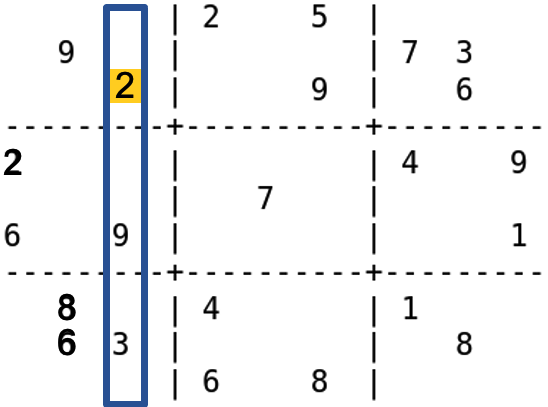
\includegraphics[width=0.7\textwidth]{figures/sudoku_steps/sudoku-step2}
\end{figure}
		}
				\only<3>{
				\begin{figure}[H]
	\centering
	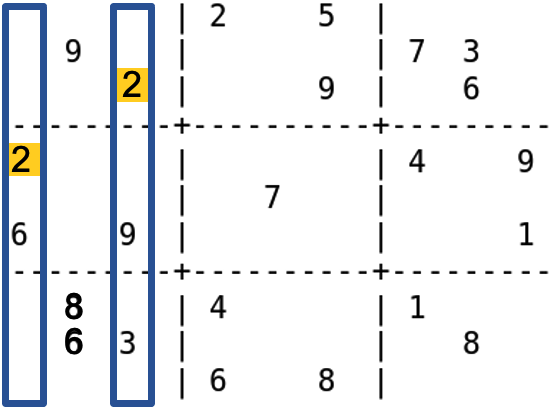
\includegraphics[width=0.7\textwidth]{figures/sudoku_steps/sudoku-step3}
\end{figure}
	}
			\only<4>{
				\begin{figure}[H]
	\centering
	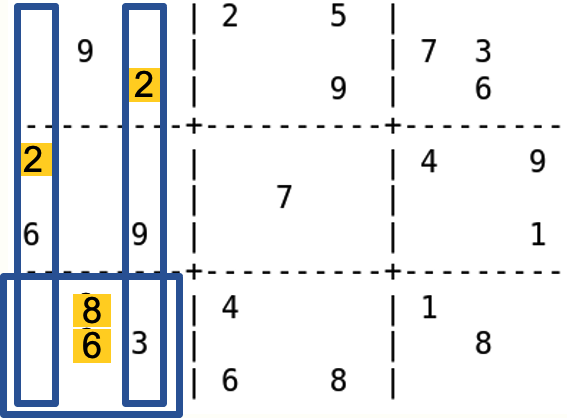
\includegraphics[width=0.7\textwidth]{figures/sudoku_steps/sudoku-step4}
\end{figure}
}
			\only<5>{
				\begin{figure}[H]
	\centering
	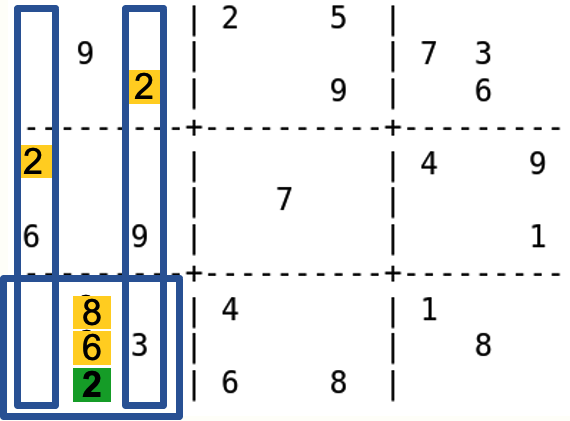
\includegraphics[width=0.7\textwidth]{figures/sudoku_steps/sudoku-step5}
\end{figure}
}
	\end{frame}

\begin{frame}
	\frametitle{Stepwise explanations for CSPs}
	\frametitle{What is a \emph{sequence} of explanations ?}
	
	\begin{minipage}{0.28\textwidth}
		\includegraphics[width=\textwidth]{figures/sudoku_sequence/sudoku-step1}
	\end{minipage}\hfill\pause
	\begin{minipage}{0.045\textwidth}
		\begin{center}
			$\rightarrow$
		\end{center}
	\end{minipage}\hfill
	\begin{minipage}{0.28\textwidth}
		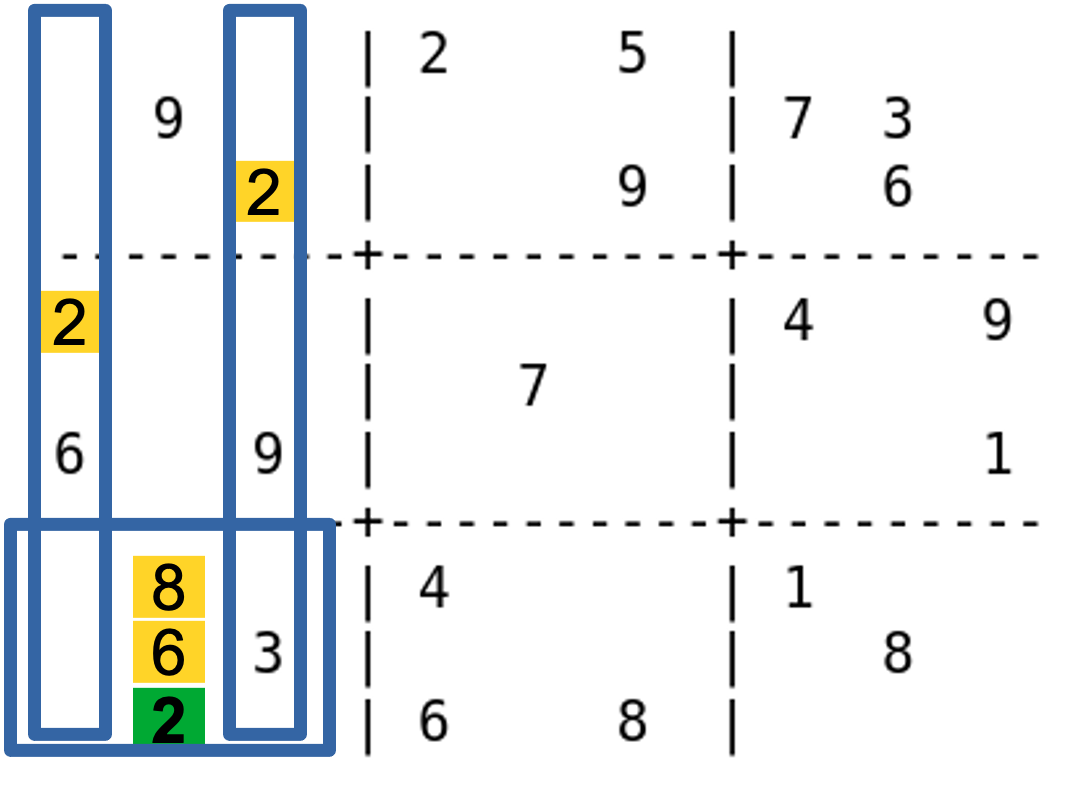
\includegraphics[width=\textwidth]{figures/sudoku_steps/sudoku3}
	\end{minipage}\hfill
	\begin{minipage}{0.045\textwidth}
		\begin{center}
			$\rightarrow$
		\end{center}
	\end{minipage}\hfill
	\begin{minipage}{0.28\textwidth}
		\begin{center}
			$\dots$
		\end{center}
	\end{minipage}\\\vfill \pause
	\begin{minipage}{0.28\textwidth}
		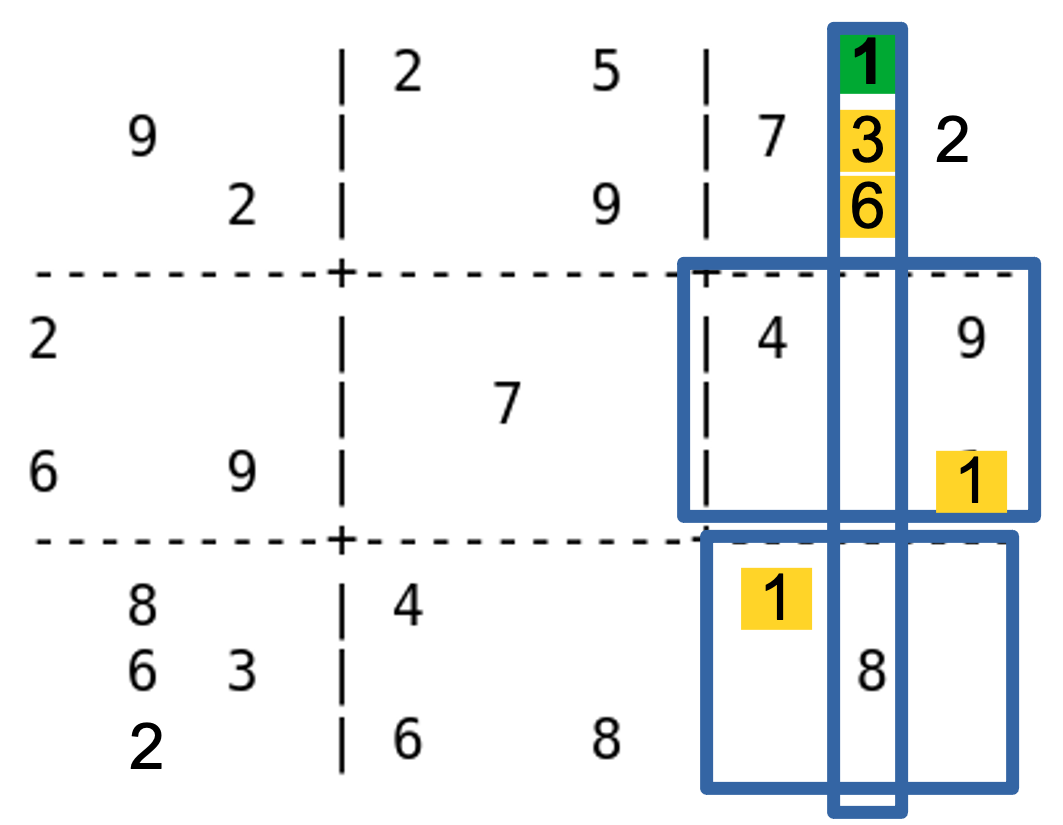
\includegraphics[width=\textwidth]{figures/sudoku_sequence/sudoku-step3}
	\end{minipage}
	\hfill
	\begin{minipage}{0.43\textwidth}
		\begin{center}
			$\rightarrow$ \hspace{0.5cm}\dots \hspace{0.5cm}$\rightarrow$
		\end{center}
	\end{minipage}\hfill\pause
	\begin{minipage}{0.28\textwidth}
		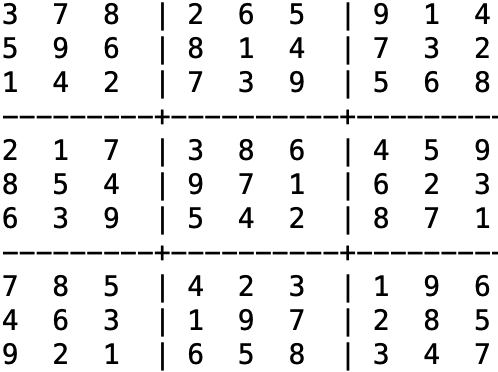
\includegraphics[width=\textwidth]{figures/sudoku_sequence/sudoku-stepn}
	\end{minipage}
\end{frame}

\begin{frame}
	\frametitle{Stepwise explanations for CSPs}
	\framesubtitle{Goal}

\textbf{Given}
\begin{itemize}
	\item[{
\includegraphics[width=15pt]{figures/explanation_steps/explanation_S_full}}] Constraints 
	\item[{
\includegraphics[width=15pt]{figures/explanation_steps/explanation_E_full}}] Facts: variable assignments ($\mathtt{cells[4,1] = 2}$), domain-reduction $\mathtt{cells[4,1] \neq 3}$
\end{itemize} \pause
\vspace{20pt}
\textbf{Goal:}
\begin{itemize}
	\item[$\triangleright$] Generate a \textit{\emph{sequence}} of \textit{\emph{simple}} explanations \pause
	\item[$\triangleright$] Explain 1 fact at a time 
	\item[$\triangleright$]  Explain step-by-step the solution of a Constraint Satisfaction Problem \pause 
\end{itemize}

\end{frame}

	\begin{frame}{Stepwise explanations for CSPs}
		\framesubtitle{Explanation step - Formal definition}

      	Let an \emph{EXPLANATION STEP} (\citet{bogaerts2020step})  be:
      	\begin{center}
      		{\Large {
\includegraphics[width=15pt]{figures/explanation_steps/explanation_E}} $\wedge$ {
\includegraphics[width=15pt]{figures/explanation_steps/explanation_S}} $\implies$ {
\includegraphics[width=15pt]{figures/explanation_steps/explanation_N}}}
      	\end{center}
      	
      \begin{minipage}{0.65\textwidth}
      	\only<1>{\hfill}
      	\only<2->{
      	\begin{itemize}
      		\item[{
\includegraphics[width=15pt]{figures/explanation_steps/explanation_E}}] A subset of previously derived facts 
\includegraphics[width=10pt]{figures/explanation_steps/explanation_E_full} 
      		\begin{itemize}
				\item[\textit{(Sudoku)}] $V_{(4, 1)}  = 2, V_{(3, 3)}  = 2, V_{(7, 2)}  = 2,V_{(8, 2)}  = 2$
      		\end{itemize}
      	\only<3->{
      		\item[{
\includegraphics[width=15pt]{figures/explanation_steps/explanation_S}}] A minimal subset of the problem constraints 
\includegraphics[width=10pt]{figures/explanation_steps/explanation_S_full}
      		\begin{itemize}
				\item[\textit{(Sudoku)}] $\{\mathtt{alldifferent}(cells[:, 1])$, $\mathtt{alldifferent}(cells[:, 3])$, $\mathtt{alldifferent}(cells[7:9, 1:3])$ 
			\end{itemize}}
		\only<4->{
      		\item[{
\includegraphics[width=15pt]{figures/explanation_steps/explanation_N}}] A newly derived fact s.t.       		{ {
\includegraphics[width=7pt]{figures/explanation_steps/explanation_E}} $\wedge$ {
\includegraphics[width=7pt]{figures/explanation_steps/explanation_S}} $\implies$ {
\includegraphics[width=7pt]{figures/explanation_steps/explanation_N}}}
      	      	\begin{itemize}
      		\item[\textit{(Sudoku)}]  $V_{(9, 2)}  = 2$
      	\end{itemize}
      }

      	\end{itemize}}
      \hfill
      \end{minipage}
        \begin{minipage}{0.3\textwidth}
			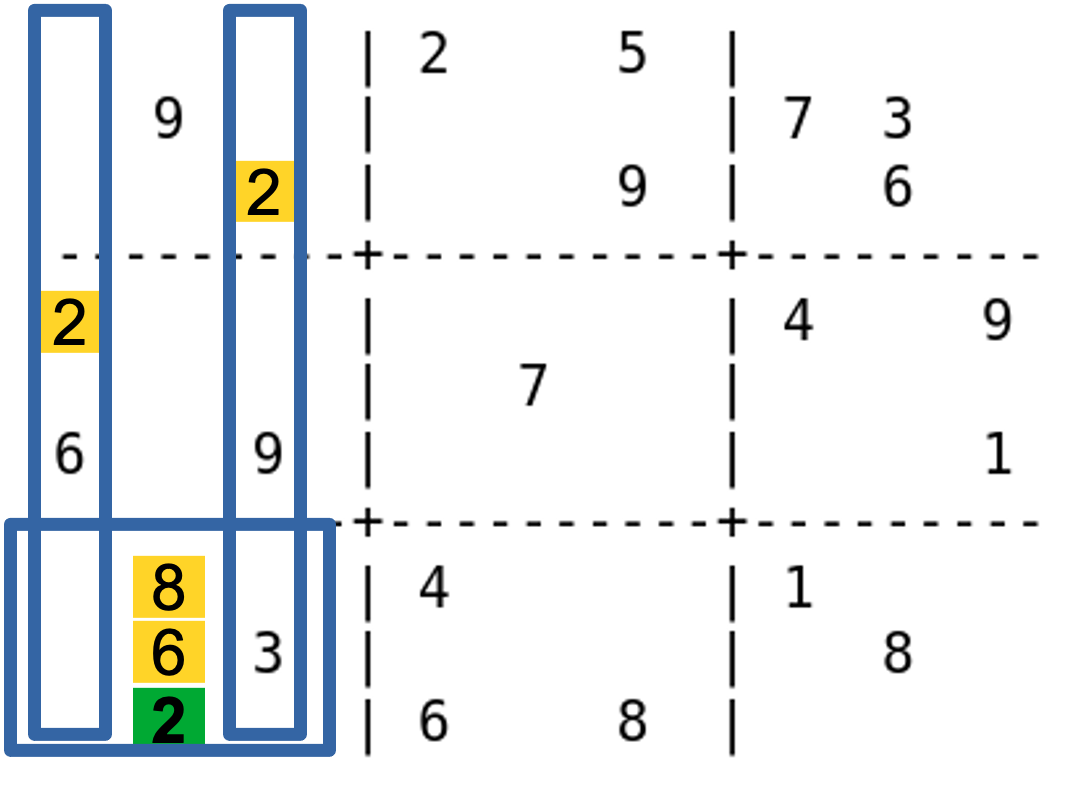
\includegraphics[width=\textwidth]{figures/sudoku_steps/sudoku3}
  \end{minipage}

      	\vfill
\only<5->{
\begin{center}
{\Large \textbf{How ?} \pause \large $\mathtt{\mathbf{MUS}}($ 
\includegraphics[width=10pt]{figures/explanation_steps/explanation_E_full} $\wedge$ {
\includegraphics[width=10pt]{figures/explanation_steps/explanation_S_full}} $\wedge \lnot$ {
\includegraphics[width=10pt]{figures/explanation_steps/explanation_N}} $)$ \textbf{is a valid explanation step}}
\end{center}
\vfill
}

	\end{frame}
	
%	\begin{frame}{Stepwise explanations for CSPs}
%		\framesubtitle{EXPLANATION STEP}
%		%		In, we introduce \emph{explanation} steps \pause
%		
%		\begin{example} (Sudoku)
%			Let $E$ contain the assigned variables at the current state of the grid (e.g. $I = \{V_{(3, 3)}  = 2, \dots \}$).
%			
%			\begin{minipage}{0.63\textwidth}
%				{\Large $\mathtt{\mathbf{MUS}}($}{\large 
\includegraphics[width=10pt]{figures/explanation_steps/explanation_S_full} $\&$ {
\includegraphics[width=10pt]{figures/explanation_steps/explanation_E_full}} $\& \lnot$ {
\includegraphics[width=10pt]{figures/explanation_steps/explanation_N}} $)$ } \\ 
%				
%				$\{\mathtt{alldifferent}(\{V_{(r,1)} | r \in {1 .. 9}\}), V_{(4, 1)}  = 2$,\\
%				$\mathtt{alldifferent}(\{V_{(r,3)} | r \in {1 .. 9}\}), V_{(3, 3)}  = 2$, \\  
%				$\mathtt{alldifferent}(\{ V_{(r_i ,c_j)} | r_i  \in 7..9 ,  c_j \in 1..3 \})$,\\  
%				$V_{(7, 2)}  = 2,V_{(8, 2)}  = 2, 	 V_{(9, 2)}  \neq 2\} $
%			\end{minipage}
%			\begin{minipage}{0.36\textwidth}
%				\begin{figure}[H]
%					\centering
%					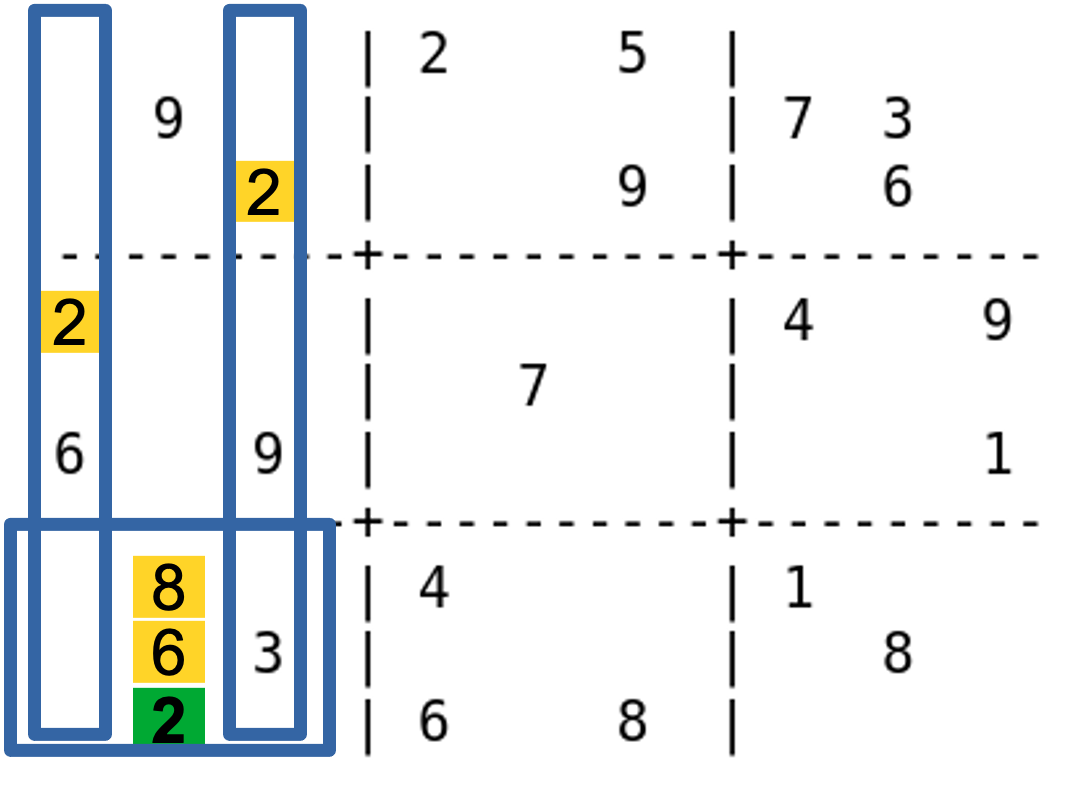
\includegraphics[width=\textwidth]{figures/sudoku_steps/sudoku3}
%					\caption{Example of a non-redundant explanation for $V_{(9, 2)}  = 2$}
%					%	\caption{Non-redundant explanation for $V_{(9, 2)}  = 2$}
%					\label{fig:example-explanation}
%				\end{figure}
%				
%			\end{minipage}
%			
%			
%		\end{example}
%		
%	\end{frame}


					\begin{frame}%{Use cases}
	\begin{center}\Large
		What are use-cases of step-wise explanations ? 
	\end{center}
	\begin{figure}
		\centering
		
\includegraphics[width=0.2\textwidth]{figures/i_want_you_ocus.png}
	\end{figure}\pause
	\begin{itemize}
		\item Explaining solutions of scheduling, configuration problems .... and puzzles  \Cooley
%		\item Debugging \textit{unsatisfiable models} with \emph{preferences} on the constraints \pause
		\item Stepwise explaining unsatisfiability \pause	
		\item Explaining Optimality for Constraint Optimization Problems 
		\begin{itemize}
			\item Why is the objective value not better ? 
		\end{itemize}
		
	\end{itemize}
\end{frame}

				\section{Toward human-interpretable explanations using Machine Learning}


		 \begin{frame}
	\tableofcontents[currentsection]
\end{frame}			

	\begin{frame}
	\frametitle{What is a \emph{good} explanation ?}
	
	%			\textbf{What is a \emph{good} explanation ?} \\ \vspace{20pt}
	\begin{minipage}{0.25\textwidth}
		\includegraphics[width=\textwidth]{figures/sudoku_sequence/sudoku-step1.png}
	\end{minipage} \pause $\rightarrow$
	\begin{minipage}{0.28\textwidth}
		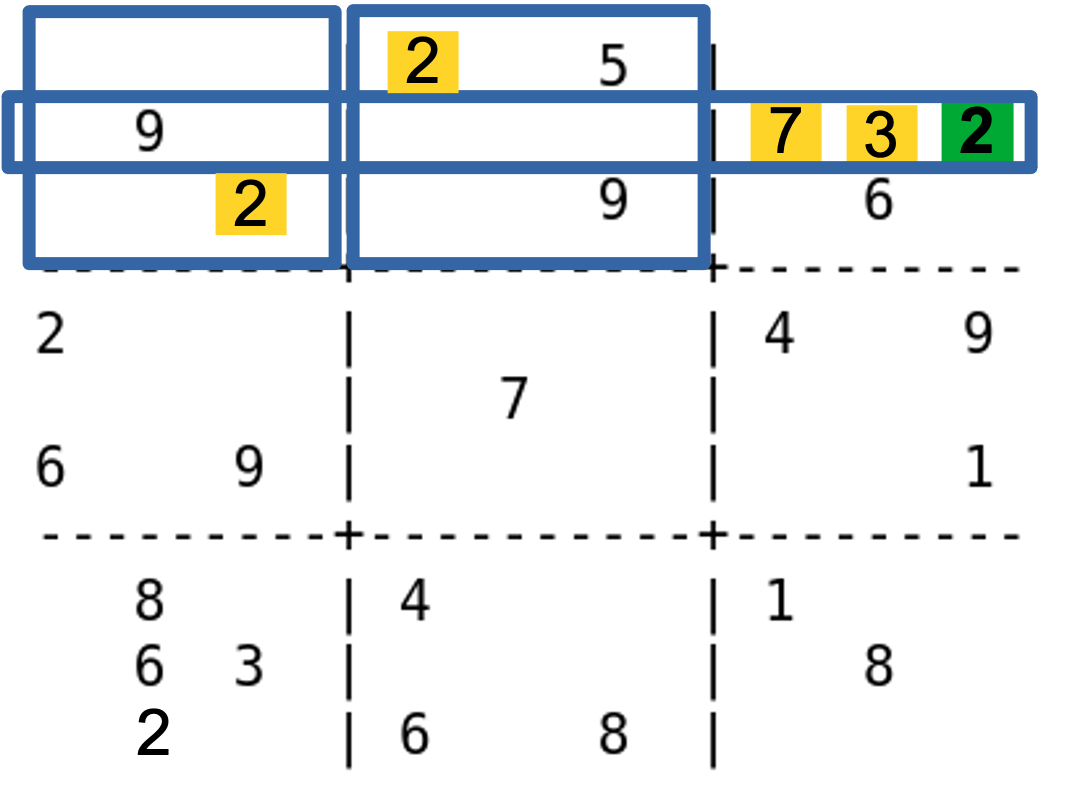
\includegraphics[width=\textwidth]{figures/sudoku_sequence/sudoku-step2}
	\end{minipage}\hfill \pause
	or \hfill
	\begin{minipage}{0.30\textwidth}
		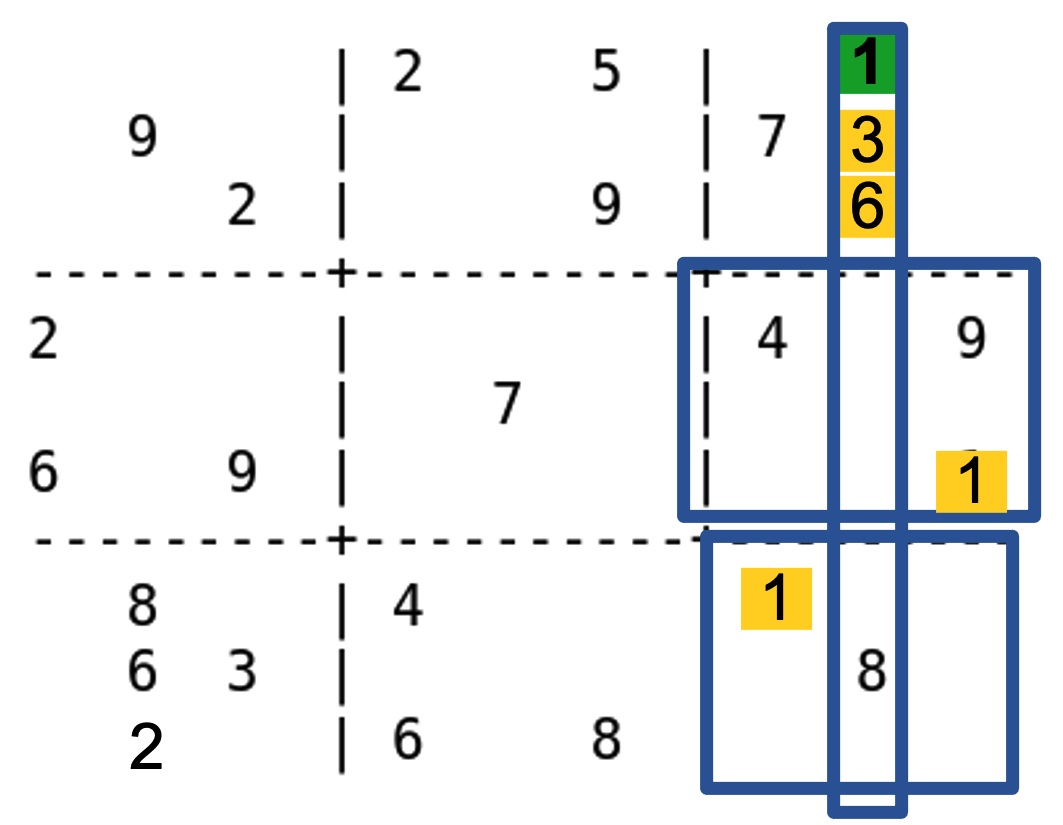
\includegraphics[width=\textwidth]{figures/sudoku_sequence/sudoku-step3bis}
	\end{minipage}
\end{frame}	


	\begin{frame}
	\frametitle{The best/easiest explanation step...}
	%		\begin{center} 
		\textbf{What is a \emph{good} explanation ?} \pause \\
		
		Let $\mathbf{f}  ($ 
\includegraphics[width=10pt]{figures/explanation_steps/explanation_E}, {
\includegraphics[width=10pt]{figures/explanation_steps/explanation_S}}, {
\includegraphics[width=10pt]{figures/explanation_steps/explanation_N}} $)$ be a cost-function that quantifies how good (e.g. easy to understand) an explanation step is.
		\pause 
		
		\vspace*{1cm}
		
		\textbf{What is the \emph{best/easiest} explanation step? }\pause
		\begin{algorithm}[H]
			
			$\mathtt{expl}_{\text{best}} \gets \mathit{nil}$\;\pause
			\For{remaining assignment {
\includegraphics[width=10pt]{figures/explanation_steps/explanation_N}} to explain}{
				
				expl $\gets \mathtt{\mathbf{MUS}}($ 
\includegraphics[width=10pt]{figures/explanation_steps/explanation_E_full} $\wedge$ {
\includegraphics[width=10pt]{figures/explanation_steps/explanation_S_full}} $\wedge \lnot$ {
\includegraphics[width=10pt]{figures/explanation_steps/explanation_N}} $, f)$\; \pause
				\uIf{$f(\mathtt{expl})<f(\mathtt{expl}_{\text{best}})$}{
					$\mathtt{expl}_{\text{best}} \gets \mathtt{expl}$\;
				}
			}
			\Return{$\mathtt{expl}_{\text{best}}$} 
		\end{algorithm}
\end{frame}

\begin{frame}
	\frametitle{Preference scoring function}
		\begin{minipage}{.45\textwidth}
			\centering
			\only<1-2>{			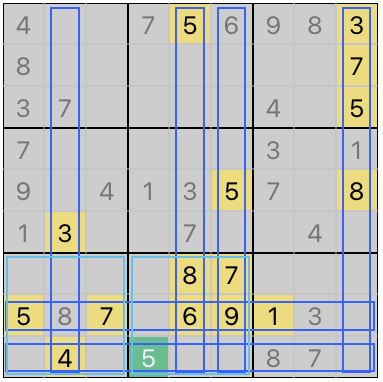
\includegraphics[width=\textwidth]{figures/overly_complicated.png}}
			\only<3>{			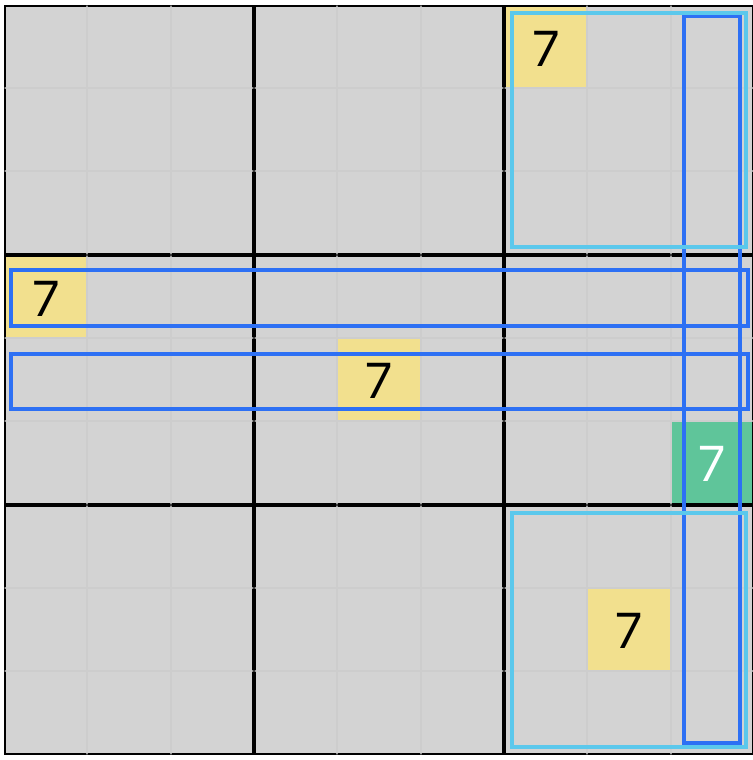
\includegraphics[width=\textwidth]{figures/explaining_7.png}}
			\only<4>{			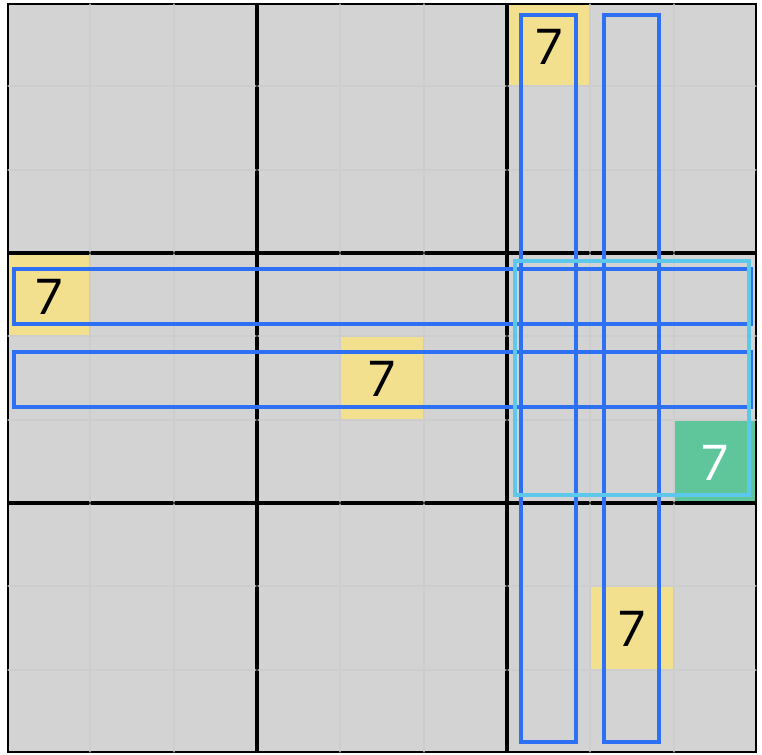
\includegraphics[width=\textwidth]{figures/explaining_7_better.png}}
		\end{minipage}\hfill	
		\begin{minipage}{.45\textwidth}
			\only<2->{
			Previous work:
			\begin{itemize}
				\item Number of constraints
				\item Number of facts
			\end{itemize}
		}
					\only<3->{New:
			\begin{itemize}
				\item Value explained
				\only<4>{
				\item Constraint graph distance
				\item Manhattan distance
				\item ... ?}
			\end{itemize}}
		\end{minipage}
\end{frame}



\begin{frame}
\frametitle{Preference learning methodology}
\begin{figure}
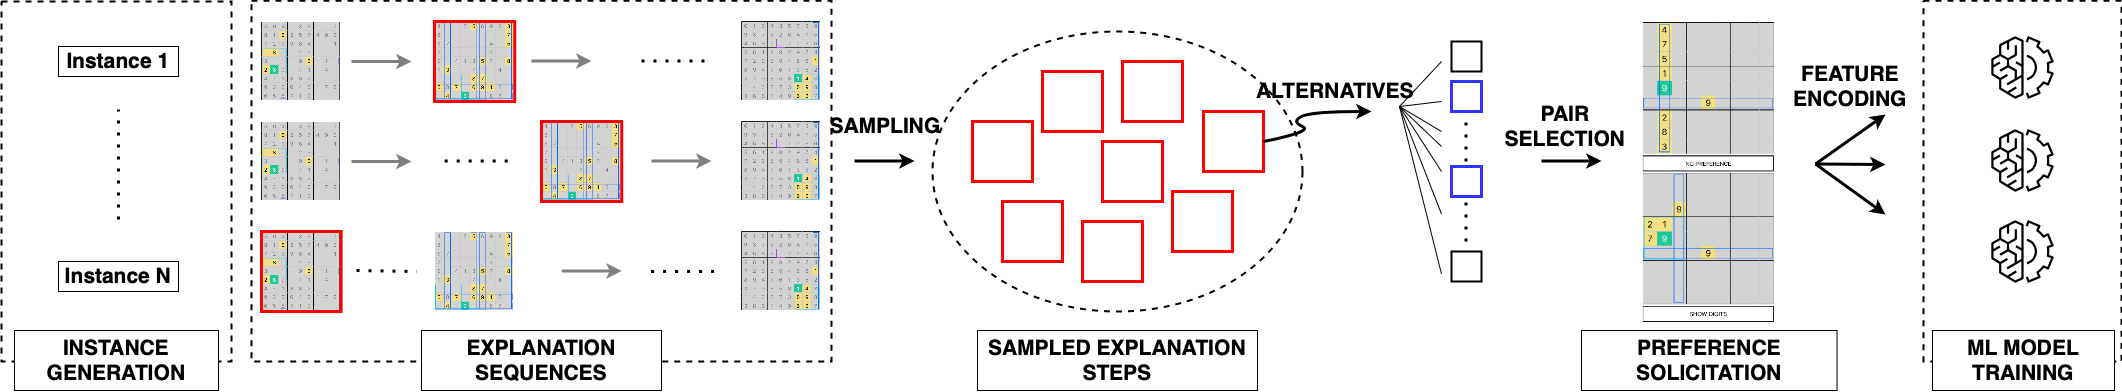
\includegraphics[width=\textwidth]{figures/cp23_preference_learning_pipeline.png}
\end{figure}
\end{frame}


\begin{frame}
\begin{table}[!h]
	\resizebox{\textwidth}{!}{
	\begin{tabular}{r|cc}
		%\toprule
		%& \multicolumn{2}{c}{\textbf{All Features}} & \multicolumn{2}{c}{\textbf{Constraints and Facts}} \\
		&  \textbf{Strict preferences} &   \textbf{All preferences} \\
		\textbf{Classifier}                   &        &        \\
		\midrule
		Hard-coded ($20*c + f$)              &    \multicolumn{2}{c}{60.58}   \\
		Logistic Regression ($w_1*c + w_2*f$) &  65.62 & \textbf{66.11}  \\
		Logistic Regression (linear features) &  63.73      &   62.10     \\ \hline
		Logistic Regression (all features) &  66.25 &  62.52 \\
		Naive Bayes                        &  59.96 &  63.21 \\
		Support Vector Machine Classifier  &  {81.76} &  79.53 \\
		Random Forest                      &  83.44 &  82.02 \\
		XGBoost                            &  \textbf{86.16} &  83.13 \\
		XGBoostRanker                      &  75.05  &  ----- \\
		%\bottomrule
	\end{tabular}}
	\caption{Classifier accuracy in predicting preferred explanation out of an explanation sample pair.}
	\label{table:classifier-accuracy}
\end{table}
\end{frame}

\begin{frame}
	\frametitle{Observations}
	\begin{itemize}
		\item A simple cost-function is better for small explanations that involve 1 constraint
		\item 
		\item 
	\end{itemize}
\end{frame}
			
		\section{Conclusion and Future work}
		 \begin{frame}
			\tableofcontents[currentsection]
		\end{frame}			
%		
\begin{frame}
	\frametitle{Conclusion and Future work}
	\begin{itemize}
		\item 
		\item 
		\item 
		\item 
	\end{itemize}
	
\end{frame}
%		
		

		
	\begin{frame}
		\frametitle{Future work}
		\begin{itemize}
			\item How to integrate the trained ML model into MUS generation to compute preferred explanation?
			\item 
		\end{itemize}
	\end{frame}
		
		
		
		\begin{frame}[allowframebreaks]
			\frametitle{References}
			\bibliographystyle{named}
			\bibliography{refs,references}
		\end{frame}		
		
		
		
	\end{document}
	
	
	
	
	
	
	
	
	
